\chapter{Implementation}
The following chapter will outline the implementation process of the project and how each component was developed. Firstly, an overview of the dataset used shall be given with information on how the images were preprocessed and augmented for training. A section for the model implementation will be given to describe how the convolutional neural network (CNN) was developed using TensorFlow. This is followed by the deployment process of the TensorFlow Python API. Lastly, the steps in which the Node.JS web application was made shall be touched upon, accompanied by the design and features choices.

\section{Data Understanding}
As stated in the system design, the dataset that will be used is the Cohn-Kanade+ image dataset, which was release in 2000 with the purpose of classifying facial expressions \citep{ck}. The dataset consists of images of 210 subject between the ages of 18 and 50. Each subject is asked to show a facial expression, beginning with a neutral facial expression that eventually lapses to the target emotion. The digital images come in either a 640x490 or 640x480 pixel format. Furthermore, the images either consists of an 8-bit grayscale or 24-bit colour format \citep{ck}. The dataset is made up of 593 image sequences and provides labels for each sequence, ranging between 0 and 6. Refer to Figure \ref{seq} for a summarized illustration of how these sequences are built.

\begin{figure}[ht]
	\begin{center}
		\advance\leftskip-3cm
		\advance\rightskip-3cm
		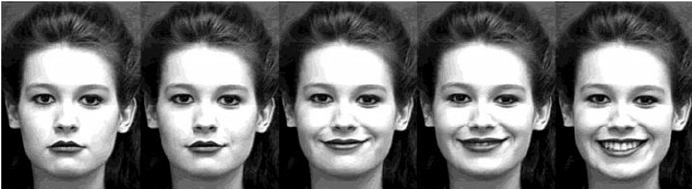
\includegraphics[keepaspectratio=true,scale=0.6]{__resources/DATASET/sequence.png}
		\caption{Image Sequence From Neutral to Happy}
		\label{seq}
	\end{center}
\end{figure}

It should be noted that the figure above is not a full image sequence and the some transitional images have been omitted. Moreover, it should also be known that there are inconsistencies in the dataset, such as a number subject not having image sequences for each certain emotions and label data missing for some images. This is acknowledged in the \textit{README} file created by Lucey et al. that is contained within the dataset, where it is declared "\textit{IF THERE IS NO FILE IT MEANS THAT THERE IS NO EMOTION LABEL (sorry to be explicit but this will avoid confusion)}". 
\section{Data Preparation and Preprocessing}
A number of preprocessing steps were taken in order to prepare the images for training the network. These steps were required to ensure maximum possible performance and minimal training time as the nature of working with neural networks can be computationally expensive when accompanied with large files such as images. The steps are as follows: Image extraction, Grayscaling, Facial Cropping, Data Augmentation and Data Splitting. 
\subsection{Image Extraction}
Due to the structure of the image sequence within the datasets, it is undesirable to used all images within each sequence as that do accurately resemble the facial expression it is used to represent. Therefore, for each sequence the last four images were extracted from their directory and relocated to a new directory under the category of facial expression they represent. As stated in the system design, images for disgust and contempt are omitted from this new dataset. Furthermore, because there is now class for a neutral facial expression, the first four images from a sequence in each subject was extracted.
The structure of the image classes for this project are as follows:
\begin{itemize}
	\item 0 - Angry
	\item 1 - Fear
	\item 2 - Happy
	\item 3 - Neutral
	\item 4 - Sadness
	\item 0 - Surprise	
\end{itemize}


\subsection{Grayscaling}
The CK+ dataset consist of a majority of gray images. However, the extended version of this dataset contains some images sequences with coloured images. When working neural networks, it is significantly more computationally expensive to process a coloured image over a gray one due to the number of colour channels. To mitigate this, a Python script was created to traverse through each image of the newly extracted dataset to convert all images to grayscale using the PILLOW library. \\

\begin{lstlisting}[language=Python, frame=single]
from PIL import Image
import numpy as np
import os, os.path
img_path = '<DATASET_DIRECTORY>' 

def grayify(file_name):
	image = Image.open(img_path + file_name)
	image = image.convert('L')
	image.save(img_path + file_name)

#Load the directory and traverse over all the image files
list = os.listdir(img_path)
for file in list:
	file_n = file
	print(file_n)

\end{lstlisting}

\subsection{Facial Cropping}
Following the grayscaling of all images, dimensionality reduction was implemented on the images. This was done by cropping each image down to only the facial surface area to reduce the noise of the data and to remove any features in the backgrounds that may be learned by the network that do not represent the facial expression. To do this, a Python script was written that reads in all the images from the dataset and crop the region of the image that contains the subject faces. This was done using the OpenCV library.

\begin{lstlisting}[language=Python, frame=single]
def facecrop(image):
	face_cascade = cv2.CascadeClassifier
	('haarcascade_frontalface_default.xml')
	
	img = cv2.imread(image)
	minisize = (img.shape[1],img.shape[0])
	miniframe = cv2.resize(img, minisize)
	faces = face_cascade.detectMultiScale(miniframe)
	
	for f in faces:
		x, y, w, h = [ v for v in f ]
		cv2.rectangle(img, (x,y), (x+w,y+h),
		(255,255,255))
		sub_face = img[y:y+h, x:x+w]
		fname, ext = os.path.splitext(image)
		cv2.imwrite(fname+"_cropped_"+ext, sub_face)
	return

list = os.listdir(<DIRECTORY_NAME>)
for file in list:
	facecrop(<DIRECTORY_NAME> + '/' + file)
\end{lstlisting}
\newpage
This was done for all images, however, some images were not correctly cropped due to noise in the image causing it to misclassify the facial region. Some examples of this might be only half the face being cropped into the new image or just the subjects shoulder being visible. These worthless images were manually deleted after the newly cropped images were evaluated. Please refer to Figure \ref{crop} for example of the facial cropping.

\begin{figure}[ht]
	\begin{center}
		\advance\leftskip-3cm
		\advance\rightskip-3cm
		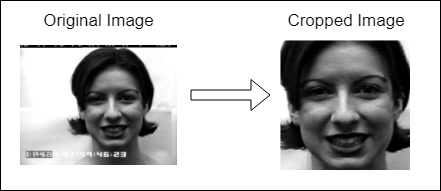
\includegraphics[keepaspectratio=true,scale=0.9]{__resources/DATASET/crop.png}
		\caption{Image Cropping on Facial Regions}
		\label{crop}
	\end{center}
\end{figure}
\newpage


\subsection{Image Increasing Through Data Augmentation}
Upon inspection of the dataset, in regards to the number of images for certain facial expressions, it was noted that there was an insufficient amount of images to train the network. This can be seen in table \ref{table: count}. 
\begin{table}[ht]
	\begin{tabular}{ |p{10cm}||p{3cm}|}
		\hline
		\textbf{Facial Expression} & \textbf{Cardinality}\\
		\hline
		\hline
		Anger & 601 \\
		\hline
		Fear & 427	\\
		\hline
		Happy & 883\\
		\hline
		Neutral & 668\\
		\hline
		Sad & 641	\\
		\hline
		Surprise  & 639	\\
		\hline
		\textbf{Total}  & \textbf{3879}	\\
		\hline
	\end{tabular}
	\caption{Initial Image Count}
	\label{table: count}
\end{table}

The initial step to increase the size of the data set was to flipped versions of all the images. Not only does this double the size of the dataset, but helps the network to better handle facial variance when dealing with new unseen data \citep{LOPES}. Also, it will decrease the chance of under-fitting while training the model. Following this step, a check was done on the class balance. Using the Matplotlib Python library, the balance of each class was plotted by counting each image in accordance to its respective label, as seen in Figure \ref{imbal} which shows the cardinality for each training sample.

\begin{figure}[ht]
	\begin{center}
		\advance\leftskip-3cm
		\advance\rightskip-3cm
		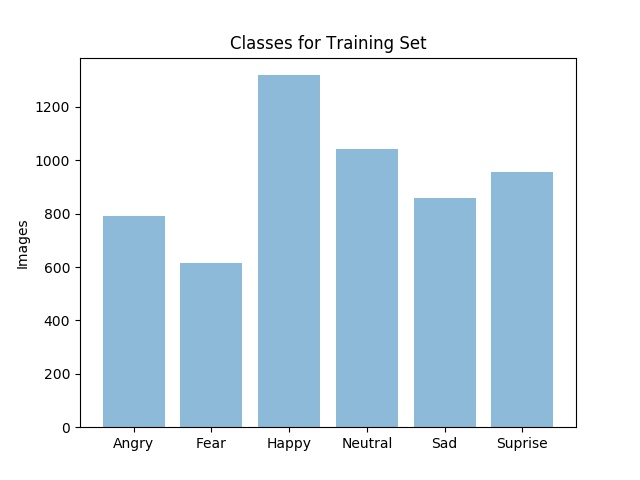
\includegraphics[keepaspectratio=true,scale=0.6]{__resources/implementation/imbalance.jpg}
		\caption{Class Imbalance}
		\label{imbal}
	\end{center}
\end{figure}\newpage
As seen above, expression 'Anger' and 'Fear' are under represented while 'Happy' is overly represented, relative to the rest of the dataset. How this problem was addressed was by creating synthetic sample images from the existing ones by the means of skewing and augmenting the images. This can be seen in Figure \ref{augm}, where the top row displays the original cropped images, and beneath, are the slightly skewing images. This was implemented using a Python library called Augmentor, which allows you to specify the directory and number of altered samples you would like, and it randomly picks images within the directory, creating an entirely new back of images that have been stretched to a degree.
\begin{figure}[ht]
	\begin{center}
		\advance\leftskip-3cm
		\advance\rightskip-3cm
		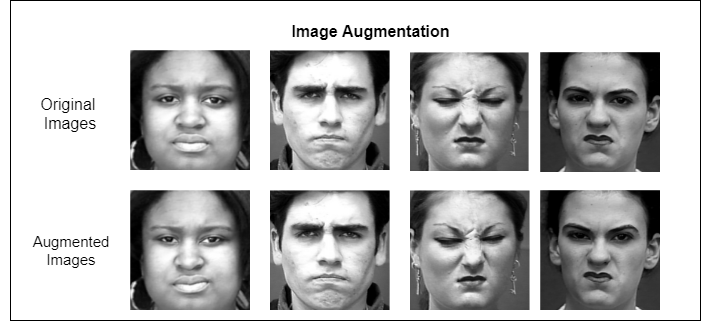
\includegraphics[keepaspectratio=true,scale=0.6]{__resources/implementation/augmented-images.png}
		\caption{Example of Augmented Images}
		\label{augm}
	\end{center}
\end{figure}
\newpage

This was done for all classes to increase the number of samples in the dataset, until a number of 1750 images are present for each class. This amounts to a total number of 10500 images in total across the entire dataset.  The class balance can be seen in the bar chart illustration in Figure \ref{bal}, which has been plotted using the Matplotlib library. In conclusion, an additional 6,621 images have been created from the original dataset.


\begin{figure}[ht]
	\begin{center}
		\advance\leftskip-3cm
		\advance\rightskip-3cm
		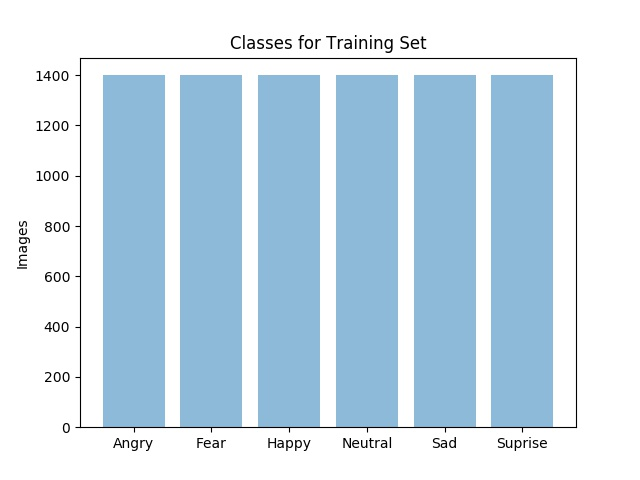
\includegraphics[keepaspectratio=true,scale=0.6]{__resources/implementation/balance.jpg}
		\caption{Class Balance}
		\label{bal}
	\end{center}
\end{figure}

\newpage

% show bad imbalance 
%flipping + synthethic examples
% show balance
\subsection{Data Splitting}
The last step in the preparation phase was to apply split validation to the dataset. The dataset was split into training and testing sets at a divide of 80/20 - meaning 80\% of the dataset will be used for training (1400 images per class) and 20\% will be used for testing the model (350 images per class). Please see the Python code below showing how this was achieved.

\begin{lstlisting}[language=Python, frame=single]
import os, os.path
import math
from PIL import Image

old_path = 'C:/Users/aaron/Desktop/Cropped Dataset/happy/'

new_train_path ='C:/Users/aaron/Desktop/data/training/happy/'
new_test_path = 'C:/Users/aaron/Desktop/data/testing/happy/'

#Load the directory and traverse over all the image files
list = os.listdir(old_path)

# define the size of the first 80 percent of images
num_files = len(list)
num_training_files = num_files * .8
num_training_files = math.ceil(num_training_files)

num_testing_file = num_files * .2
num_testing_file = math.ceil(num_testing_file)

#Add the first 80 percent to the training folder
for img in list[1:num_training_files]: 
	i = Image.open(old_path + img)
	i.save(new_train_path+img)


#Add the remaining 20 percent to the training folder
for img in list[num_training_files:]:
	i = Image.open(old_path + img)
	i.save(new_test_path+img)
\end{lstlisting}

\section{Implementing the Machine Learning Model}

When implementing the machine learning model with TensorFlow, the initial step used is to import all the libraries that deemed necessary for preprocessing and training. These include TensorFlow, Numpy, Skimage, PIL etc. Secondly, the image data was imported. A list is used to store the image RGB data for every image in the dataset. Secondly, as stated in the data understanding, there is some inconsistency in the dataset such as some images not being labeled. Therefore, the class folder in which a certain image is imported from was used as the label, and added to the labels list. Refer code below to see how this was implemented.

\begin{lstlisting}[language=Python, frame=single]
def load_data(TRAINING_DIR):
images = []
labels = []

directories = [d for d in os.listdir(TRAINING_DIR) 
if os.path.isdir(os.path.join(TRAINING_DIR, d))]

# Traverse through each directory and make a list
# of files names if they end in the PNG format
for d in directories:
	label_directory = os.path.join(TRAINING_DIR, d)
	file_names = [os.path.join(label_directory, f) 
	for f in os.listdir(label_directory) 
				if f.endswith(".png")]
	
	#Traverse through each file, add the image data
	# and label to the 2 lists
	for f in file_names:
		images.append(skimage.data.imread(f))
		labels.append(int(d))
	return images, labels

images, labels = load_data(TRAINING_DIR)
\end{lstlisting}

Following this, shuffling of the data is performed, this is done to prevent overfitting of the model. Then each image in the list of images are sub sampled from their original sizes down to a 50x50 pixel size. This was done with the Skimage library to reduce the dimensionality of the images for the network to better handle the input data. The list images were traversed and resized using the transform function. 
\begin{lstlisting}[frame=single]
images = [transform.resize(image,(50, 50))
	for image in images]
\end{lstlisting}

After the basic data imports and preprocessing, defining the computation graph for TensorFlow is required. TensorFlow placeholder were then declared for later use when tensors need to be fed to the TensorFlow session, along with another few initial variables such as number of epochs, the batch size, dropout rate etc. When all the main variables needed for TensorFlow are made, the structure of the network was mad. This was done using the tf.slim library, which a TensorFlow package that allows you to define layers in a network easily. 

In total there are 10 convolution layers with 5 Max Pooling layers. The convolution layer is used to extract features within the image while pooling reduces the dimensionality of the feature maps, but retains majority of the useful data. Please refer to Figure \ref{map}

\begin{figure}[ht]
	\begin{center}
		\advance\leftskip-3cm
		\advance\rightskip-3cm
		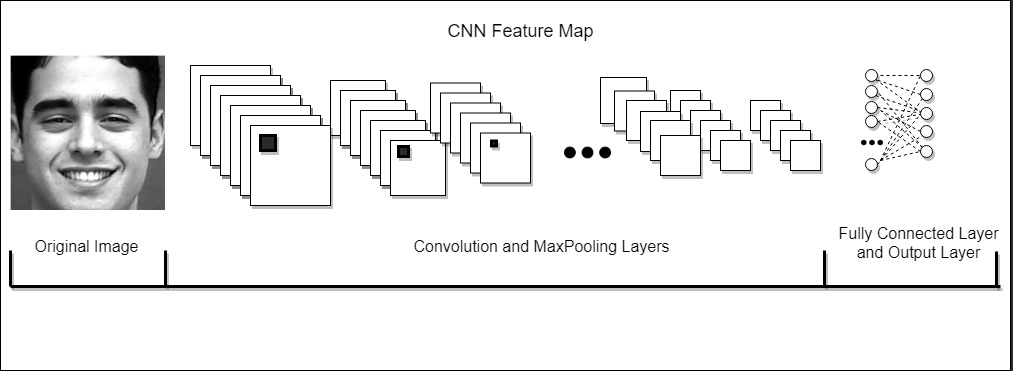
\includegraphics[keepaspectratio=true,scale=0.48]{__resources/implementation/map.jpg}
		\caption{Feature Maps of CNN}
		\label{map}
	\end{center}
\end{figure}

Lastly, a fully connected layer is defined, which will be used to produce a predicted output. Dropout is a regularization technique that is used in this case is to reduce the chances of over fitting the network \citep{JMLR}. After each training iteration (epoch), only 80 percent of the trained neurons are kept.\\ \\

\begin{lstlisting}[language=python, frame=single]
	net = slim.conv2d(net, 32, 3)
	net = slim.conv2d(net, 64, 3)
	net = slim.conv2d(net, 64, 3)
	net = slim.max_pool2d(net, 3, stride = 1 )
	net = slim.conv2d(net, 96, 3)
	net = slim.conv2d(net, 96, 3)
	net = slim.max_pool2d( net, 2, stride = 2)
	
	net = slim.conv2d(net, 128, 3)
	net = slim.conv2d(net, 128, 3)
	net = slim.max_pool2d( net, 2, stride = 2)
	
	net = slim.conv2d(net, 128, 3)
	net = slim.conv2d(net, 128, 3)
	net = slim.max_pool2d(net, 2, stride = 2)
	
	net = slim.conv2d(net, 128, 3)
	net = slim.max_pool2d(net, 2, stride = 1)
	
	net = slim.dropout(net, keep_prob = keep_rate
		, is_training = is_training )
\end{lstlisting}

Following the structure set up of the network, a function is defined that runs the TensorFlow session, which takes the \textbf{x} placeholder as a parameter.
Within this function we define the loss function used within the network which is softmax with cross entropy. Also, the Adam optimizer is used for back propagating through the network and adjusting the weights. The Adam optimization algorithm is said to be a suitable optimizer to use as it is very robust when dealing with high dimensionality \citep{DBLP}. Which, in the case of a CNN, is highly preferable. A learning rate of 0.002 was chosen for the final implementation after showing in experimentation that this reduced the loss the most. 

\begin{lstlisting}[language=python, frame=single]
loss = tf.reduce_mean(tf.nn.softmax_cross_entropy_with_logits
    (labels = y, logits = output))
total_losses = tf.losses.get_total_loss
	( add_regularization_losses=True ) + loss

update_ops = tf.get_collection(tf.GraphKeys.UPDATE_OPS)
with tf.control_dependencies(update_ops):
train_op = tf.train.AdamOptimizer( learning_rate=0.002 )
			.minimize( total_losses )
\end{lstlisting}


When the session is ran, the TensorFlow variables are initialized and the training begins. 
The list of images and labels are segmented into batches of size 100 to prevent an OOM error, as loading all the images into memory can cause an overflow. The images and labels are fed into the TensorFlow runtime environment for training. After each epoch, the accumulated loss and batch accuracy is calculated and printed to the screen.
After the network have been trained for the specified number of epochs, it evaluated the accuracy on the test data and a TensorFlow \textit{.CKPT} model file is saved to disk.

\begin{lstlisting}[language=python, frame=single]
op, ac, loss_value, total_loss_value, pred_classes, 
label_classes = sess.run([train_op, acc, loss, total_losses,
 pred_class, label_class ], 
feed_dict={x: train_batch_x, y: train_batch_y,
 is_training : True})
\end{lstlisting}


% Image images
% preprocessing
% Create comptation graph
% create session

\section{Deploying the Trained Model}
% 1 - Flask API
In order to deploy the trained TensorFlow model a Python application programming interface was created using the Flask library. Flask is a microframework developed for running Python scripts on a server, similar to Node.js and Express. In the API, routes were set up to handle HTTP POST requests. When image data in the form of Base64 is sent to the server, it is decoded from Base64 and written to disk in the form of a PNG file. This file is then preprocessed to have the same characteristics as the data the model was trained on. The image is converted to grayscale, then resized to be 50x50 pixels and lastly a new dimension is added to the image so that it can be interpreted by TensorFlow trained model. After a classification results is returned from the model, the results is converted to a JSON string and returned to the application from which the request came.

\begin{lstlisting}[language=python, frame=single]
@app.route('/api', methods=["POST"])
@cross_origin()
def evaluate():

imageData = request.get_data()
data_preprocessing(imageData)
print('1: Image was converted')

image = Image.open('output.jpg')
image = image.convert('L')
image = image.resize((50, 50), Image.ANTIALIAS)
print('Resized and Grayscaled Image') 

image = np.expand_dims(np.array(image), axis = 0)
classification = sess.run(prediction, feed_dict = 
	{x: image, is_training : True})  
	
# add highest probability result to classes
classes = np.argmax( classification, axis = 1 )

res = 'undefined'
if   classes[0] == 0:
	print('Predicted: Angry')
	res = 'Angry'
elif classes[0] == 1:
	print('Predicted: Fear')
	res = 'Fear'
elif classes[0] == 2:
	print('Predicted: Happy')
	res = 'Happy'
elif classes[0] == 3:
	print('Predicted: neutral')
	res = 'Neutral'
elif classes[0] == 4:
	print('Predicted: sad')
	res = 'Sad'
elif classes[0] == 5:
	print('Predicted: Suprised')
	res = 'Suprised'

return jsonify(res)
\end{lstlisting}

For deployment, the Heroku PaaS was used with GitHub integrations. Whenever a commit was made to the master branch the API was automatically deployed to the server, a build is made and then the API is ready for use.


\section{Implementing the Node.JS Application}
To develop a web application for the user to interact with, Node.JS was used to implement a simple one-page application that accesses the users webcam. Firstly, a Javascript web-server was created using the Express npm module, which provides functions for routing and serving html pages. A port is initially set using either port 5000 for local development, or a randomly allocated port for a deployment environment. 

\begin{lstlisting}[language=python, frame=single]
	app.set('port', (process.env.PORT || 5000))
\end{lstlisting}

This is followed by providing the home page when the base route is called by from the client. When the \textbf{'/'} route is called, a html page containing the application is delivered to the users browser and displayed in the DOM.

\begin{lstlisting}[language=python, frame=single]
app.get('/', function (req, res) {
  res.sendFile(path.join(__dirname, '/index.html'));
});

var server = app.listen(app.get('port'), function () {
  var host = server.address().address
  console.log('Application running on port', app.get('port'))
})
\end{lstlisting}

\subsection{Facial Tracking With a Users Webcam}

The user interface design of the application is very simple. On the left hand side of the page the webcam feed is displayed. This accesses the user's machine's webcam and displays it to the screen using the html \textbf{canvas} element. Canvas is a container for drawing graphics to the page. For facial tracking, a library called Tracking.js was imported. Tracking.js is an open source library created by Eduardo Lundgren for object, colour and face detection using javascript. The reason for this library choice was because other alternatives, such as OpenCV, deemed to be very heavy weight in comparison and API services that have also been considered such as Cloudinary would reduce classification speed as it would be computationally expressive to make multiple requests for facial cropping while using the application. 
In light of this, Tracking.js provides a lightweight and quick solution for detecting faces. Using what is known as haar cascades, object classification and detection is made simplified and provides fast calculation speeds \citep{viola}. In terms of the web application, the canvas drawing of the webcam feed is read and interpreted by Tracking.js and the facial features are detected. A yellow square is drawn around the detected facial area.

\begin{lstlisting}[language=python, frame=single]
var tracker = new tracking.ObjectTracker('face');
tracker.setInitialScale(4);
tracker.setStepSize(.5);
tracker.setEdgesDensity(0.1);
tracking.track('#video', tracker, { camera: true });
tracker.on('track', function(event) {
context.clearRect(0, 0, canvas.width, canvas.height);
\end{lstlisting}

One function that tracking.js does not provide is the ability to crop the detected area of the stream. To get around this, Javascript code was developed to mark the area in which the square was being drawn around the user's face. In each frame of a user's face being detected a new square is drawn to the canvas, so every time that a new square is displayed to the screen, this marks the new coordinates of the area in which is needed for cropping. 

\begin{lstlisting}[language=python, frame=single]
rect_width = rect.width; // 
rect_height = rect.height;
rectX = rect.x;
rectY = rect.y;

 ...
ctx.drawImage(video, rectX+ 100, rectY +90,
	 rect_width +70,  rect_height +50, 0, 0, 300, 150);
\end{lstlisting}

After it is known where the users face is positioned in the shot, the cropped area is displayed in a separate 100x100 pixel canvas area, named ctx, below the feed. To ensure that the trained TensorFlow API does not become overflowed with image data, an interval timing is implemented. This involves setting a timer as to when an image is cropped because it would be disadvantageous and computationally expensive to have every frame to be sent to the API. In this case, the interval is set to 2 seconds. To initiate a session with the model and begin the facial sentiment analysis, a button was added to the UI which begins the analysis. Please refer to the Figure \ref{web} for a screenshot of the facial tracking in action.

\begin{figure}[ht]
	\begin{center}
		\advance\leftskip-3cm
		\advance\rightskip-3cm
		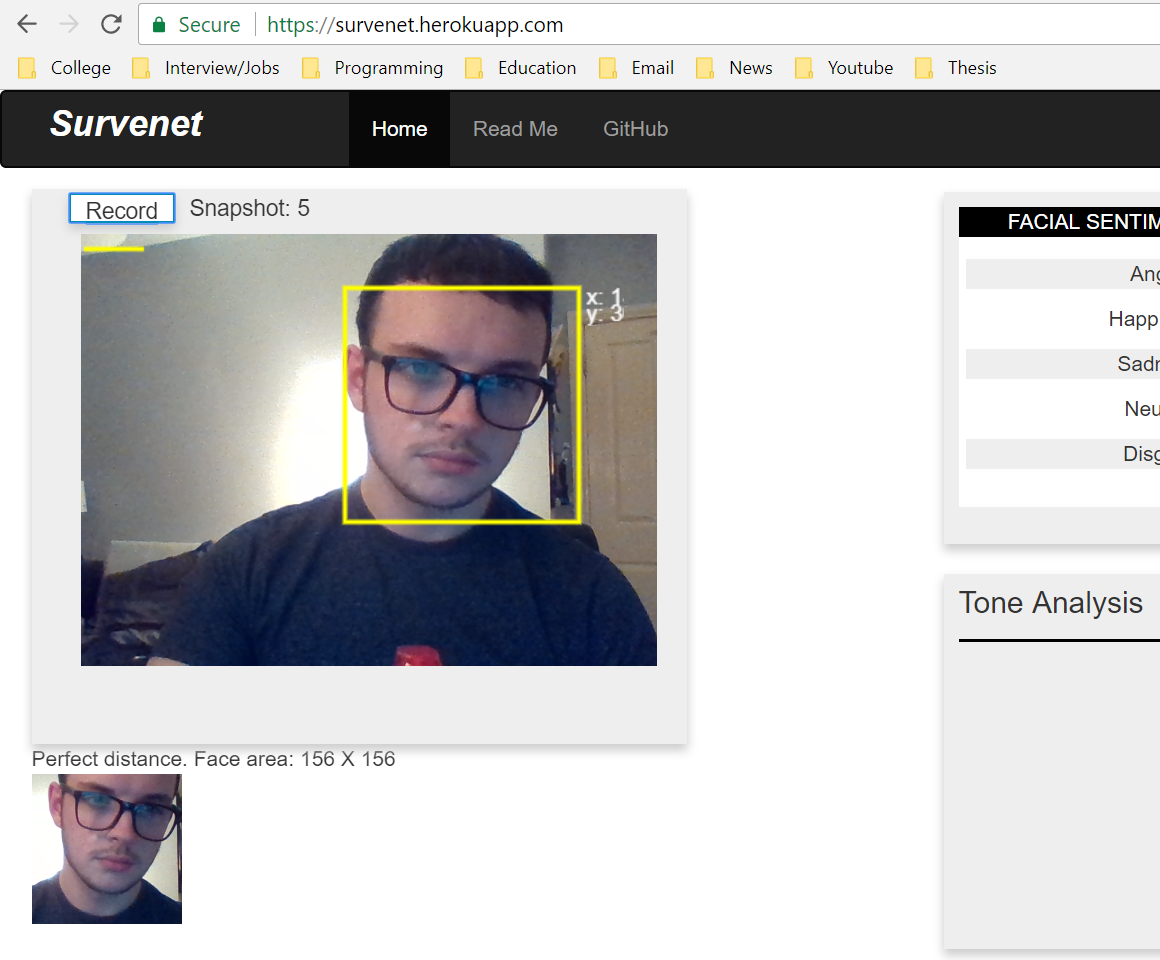
\includegraphics[keepaspectratio=true,scale=0.5]{__resources/implementation/webapp1.png}
		\caption{Webcam Feed with Facial Tracking and Cropping}
		\label{web}
	\end{center}
\end{figure}

\newpage

\subsection{Facial Sentiment Analysis} 

For each of the images sent to the model API, a classification is returned. This classification of facial expression is not only just displayed to screen, but it is used to calculate the percentage of emotions over all. To calculate the relative percentage of a certain emotion, the number of times it is classified is counted, and it is divided by the total number of classifications made. Then this result if multiplied by 100/1. Please see Equation 5.5.1.

\begin{equation}\label{eq:per}
Class percentage = 
\frac{
	number of classifications
}{
	Total number of classifications
}
X   
\frac{
	100
}{
	1
}
\end{equation}

These results are displayed to the screen and are updated constantly after each image is taken. Furthermore, when the Percentage of happiness is above 40\%, a notice is given that good customer service is being given, as shown in Figure \ref{good}.

\begin{figure}[ht]
	\begin{center}
		\advance\leftskip-3cm
		\advance\rightskip-3cm
		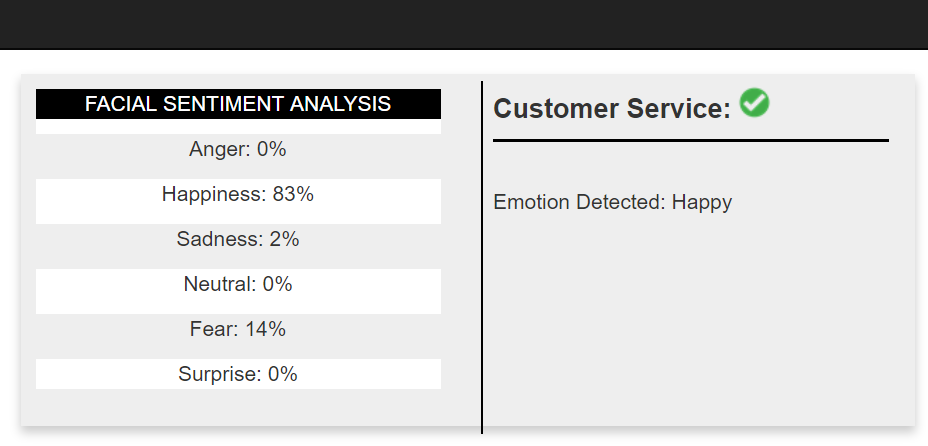
\includegraphics[keepaspectratio=true,scale=0.6]{__resources/implementation/good.png}
		\caption{Emotion Classification Metrics when Mostly Happy}
		\label{good}
	\end{center}
\end{figure}


Also, when the happiness level of the user reaches below 40\%, is is notified that poor customer service is being given. See Figure \ref{bad}

\begin{figure}[ht]
	\begin{center}
		\advance\leftskip-3cm
		\advance\rightskip-3cm
		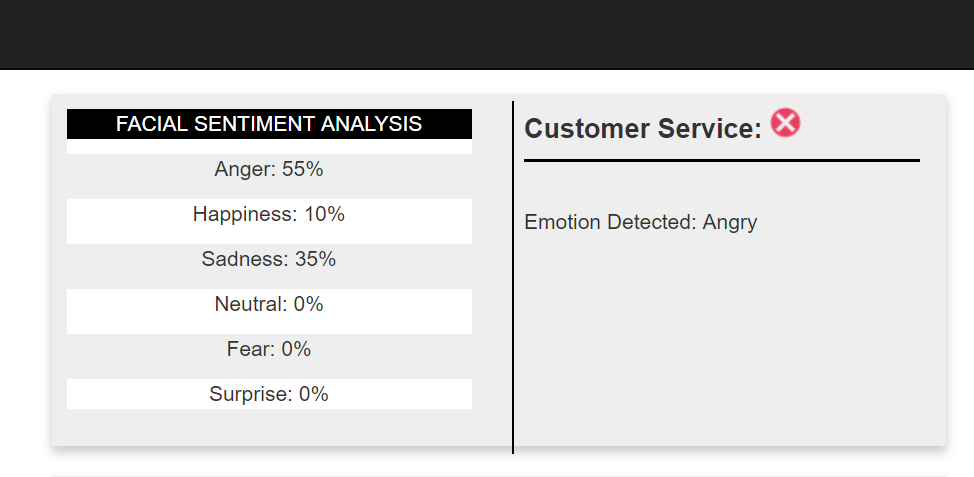
\includegraphics[keepaspectratio=true,scale=0.6]{__resources/implementation/bad.png}
		\caption{Emotion Classification Metrics when Mostly Angry}
		\label{bad}
	\end{center}
\end{figure}
\newpage

After 100 iterations of classification, the interaction stops with the model and the user is notified whether or not they have been delivering good or bad customer service.


% 1 - Create Node/express application
% 2 - Implement webcam canvas
% 3 - Apply tracking.js
% 4 - impelement facial cropping
% 5 - Make request to API

\section{Deploying the Node.JS Application}


For deploying the web application, the Heroku PaaS of service was used. Using GitHub integrations, whenever a new version of the application was pushed to the remote repository a new build was commenced. If the build was successful, the application would be live for use at \textit{https://survenet.herokuapp.com}.

%\subsection{Database Integration
%\section{Result Weighting Algorithm}
%\section{Integrating Third Party Services}
\section{Concluding Remarks of Implementation}

In summary, many data preprocessing steps were taken. These include grayscaling, facial cropping, data increase by creating flipped copies and image augmentation. These steps were taken to ensure the best possible results when evaluating the model. Secondly, the data was split into training and testing sets. A fully working TensorFlow convolutional neural network was created in Python and trained on the FloydHub could training platform. The model was then deployed to a server for production use. A facial tracking web application was built for recording the used face and deployed to the Heroku PaaS. The application can accurately calculate the level of satisfaction displayed with the used facial expression for each class.



